\documentclass[11pt,dvipdfmx,a4paper]{jsarticle}

\usepackage{amsmath,amssymb}
\usepackage{bm}
\usepackage[dvipdfmx]{graphicx}
\usepackage{physics} % http://mirrors.ibiblio.org/CTAN/macros/latex/contrib/physics/physics.pdf
\usepackage{siunitx} %SI単位を楽に出力
\usepackage{mathtools} %環境の追加
% \usepackage{circuitikz} %電気回路をtex中で書く
% \usepackage{caption} %番号なしキャプションを書く
% \usepackage{cancel} %式中に斜線を入れる
% \usepackage{tensor} %テンソルの添え字を書く
% \usepackage{tikz} %図を書く
% \usepackage{ascmac} %四角い枠の中に文章を書く
% \usepackage{float} %figureで[hbp]オプションを使う
% \usepackage{hyperref}  \usepackage{pxjahyper} %ハイパーリンクをつかう
% \usepackage{tablefootnote} %表中に注釈をいれる
% \usepackage[thicklines]{cancel} %数式中の取り消し線
\usepackage[version=4]{mhchem} %化学式の入力
\usepackage{pdfpages}
\usepackage{wrapfig} %文章の回り込み
\usepackage[subrefformat=parens]{subcaption} %(a)図のようにすることができるやつ
\usepackage{here}
\usepackage{mathrsfs} % フォントの追加
\usepackage{url} % url を入れる
\usepackage[margin=15mm]{geometry} %余白の削除

\numberwithin{equation}{section}

\graphicspath{{./image/}}

\begin{document}

%出力したpdfを表紙にするとき
% \includepdf[pages=1,noautoscale=false]{cover.pdf}
% \newpage

%texで表紙を書くとき
\quad\\[35mm]
\centerline{\Huge{\textsf{第 5 回}}}
\quad\\[5mm]
\centerline{\Huge{\textsf{応 用 物 理 学 実 験}}}
\quad\\[5mm]
\begin{table}[h]
	\centering
	\begin{tabular}{| c | c |}
		\hline
		\Huge\textsf{{題目}} & \Huge{\textsf{半導体}} \rule[-5mm]{0mm}{15mm} \\
		\hline
	\end{tabular}
\end{table}
\quad\\[10mm]
\begin{table}[h]
	\centering
	\begin{tabular}{l l}
		\hline
		\LARGE{\textsf{氏\qquad 名}} & \LARGE{\textsf{: 西原 翔}} \rule[0mm]{0mm}{6mm} \\
		\hline
		\LARGE{\textsf{学  籍  番  号}} & \LARGE{\textsf{: 1522068}} \rule[0mm]{0mm}{6mm} \\
		\LARGE{\textsf{学部学科学年}} & \LARGE{\textsf{: 理学部第一部応用物理学科3年}}\\
		\hline
	\end{tabular}
\end{table}
\quad\\[10mm]
\centerline{\LARGE{\textsf{共同実験者:1522064 中井空弥}}}\\[2mm]
\quad\\[10mm]
\centerline{\LARGE{\textsf{提出年月日:2024年07月18日}}}\\[2mm]
\centerline{\LARGE{\textsf{実験実施日:2024年06月28日}}}\\[2mm]
\centerline{\LARGE{\textsf{\qquad\qquad\quad\;2024年07月05日}}}
\quad\\[10mm]
\centerline{\LARGE{\textsf{東 京 理 科 大 学 理 学 部 第 1 部}}}\\[2mm]
\centerline{\LARGE{\textsf{応 用 物 理 学 教 室}}}

\thispagestyle{empty}
\clearpage
\addtocounter{page}{-1}
\newpage

% \twocolumn
\section{目的}

\section{原理}
\subsection*{電気伝導の古典論}
電気伝導は線形応答理論を用いて量子論的に扱うこともできる。
しかし、驚くべきことに古典論を使った議論であっても正確な議論ができる。
この節では電気伝導のオームの法則とホール効果を古典的なモデルで説明していく。
\subsubsection*{外部磁場がないときの電気伝導}
量子論以前の1900年頃、
Drudeは電気伝導について古典的なモデルを立てて議論した。
電気伝導の担い手は一種類で、外部電場\(\mathscr{E}\)中を動く質量\(m\), 電荷\(q\)を持った理想気体とみなして、
古典的な運動方程式で記述する。
電子気体は様々な要因によって散乱されるものとして、
運動方程式を立てると、
\begin{equation}
    m\dot{v} + \frac{m}{\tau}v= q\mathscr{E}.
\end{equation}
このときの\(v_D\)はドリフト速度というもので電子の速度から
電場のない熱平衡状態における電子の速度\(v_{\text{therm}}\)
を用いて
\(
    v_D= v-v_{\text{therm}}
\)
と表されるものである。
電場がないときこの古典的な運動方程式の解は
\begin{equation}
    v = v_{\text{therm}}\qty(1-e^{-t/\tau})
\end{equation}
である。
電場があるときには解は\(v_{\text{therm}}\)が十分小さいと考えて、
\begin{equation}
    v = \frac{q\mathscr{E}\tau}{m}\qty(1-e^{-t/\tau}).
\end{equation}
するとドリフト速度は
\begin{equation}
    v_D=\frac{q\tau}{m}\mathscr{E}
\end{equation}
となる。
電流密度はこのドリフト速度を用いて次のように表せる。
\begin{equation}
    j = qnv_D = \frac{q^2\tau n}{m}\mathscr{E} = qn\mu\mathscr{E}
\end{equation}
このとき\(n\)は自由電子の体積密度、
\(\mu\)は移動度\footnote{易動度とも書いたりする。英語では mobility というので易動度の方が字が合っているが移動度の方が多く使われている。}
と呼ばれる量で、
\begin{equation}
	\mu = \frac{q\tau}{m}
\end{equation}
というようになる。この量はキャリアの電荷が大きければ大きいほど、
散乱する時間間隔が長ければ長いほど、キャリアの重さが軽ければ軽いほどキャリアが動きやすいということを表している。
そして、キャリアの持つ電荷の符号も反映している量になっている。

また外部電場と電流密度が比例していることがわかる。
これをオームの法則という。
比例定数を電気伝導度\(\sigma\)といい、
\begin{equation}
	\sigma := \frac{j}{\mathscr{E}} = qn\mu = \frac{q^2n\tau}{m}
\end{equation}
となる。またこれの逆数は抵抗率\(\rho\)と言われる。
この式で注目すべきことは散乱の度合い\(\tau\)やキャリアの電荷の大きさ\(e\), 質量\(m\)が変わらなければ、
電気伝導度はキャリアの密度に比例するとみなせる点である。
なので電気伝導度を測定することでキャリア密度の測定にも使えることがわかる。

この古典論の式を実際の系に当てはめる際に注意点がいくつかある。
1つは電気伝導の担い手1種類だけではなく、電子と正孔の2種類ある点である。
これにより電気伝導度は各キャリアごとに考える必要がある。
電子密度と移動度を\(n,\,\mu_e\), 正孔密度と移動度を\(p,\,\mu_e\), 電気素量を\(e\)として
\begin{equation}
	\sigma = -en\mu_e +e p\mu_p
\end{equation}
というようにする必要がある。

2つ目はキャリアとなっている電子は準粒子の方の電子である。
そのため、質量は真空中の電子の質量ではなく有効質量の方で、
電子密度\(n\)も結晶中全ての電子ではなく準粒子の電子の数となる。

\subsubsection*{外部磁場があるときの電気伝導}
電流\(I\)が流れる方向に垂直な方向に磁場\(B\)をかけることを考える。
電流の流れる方向を\(x\)軸、磁場を書ける方向を\(z\)軸とする。
電荷\(+e\)を持った正孔は\(x\)軸の負の方向へ運動し、
電荷\(-e\)をもった電子は\(x\)軸の正の方向へ運動する。
するとローレンツ力\(F = q\vb*{v}\times\vb*{B}\)によって、
いずれのキャリアも\(y\)軸の負の方向へ偏っていく。
電子と正孔では有効質量や密度が違うため、
この電荷の片寄りはキャリアのうち移動しやすく量の多いキャリアが優勢的になる。
正孔が優勢なときには\(y\)軸の負方向にプラス電荷が多くなるため、
\(y\)軸の正の方向へ一様な電場が生じる。
一方、
電子が優勢なときには\(y\)軸の負方向にマイナス電荷が多くなるため、
\(y\)軸の正の方向へ一様な電場が生じる。
つまり、結晶中を流れるキャリアが正孔的なふるまいをするのか、
電子的な振る舞いをするのかをこの電場の符号を測定すればわかる。
このようにキャリアの符号により同じ電流の向き、同じ磁場の向きであっても電場の向きが変わる効果をホール効果という。

これを定量的に評価していく。
電場\(\mathcal{E}=(\mathcal{E}_x,\,\mathcal{E}_y,\,\mathcal{E}_z)\), 磁場\(B=(0,\,0,\,B)\)の下、
粘性抵抗のあるキャリアの運動方程式は
\begin{equation}
	m^*\dv{t}
	\begin{pmatrix}
		v_x\\
		v_y\\
		v_z
	\end{pmatrix}
	=-\frac{m^*}{\tau}
	\begin{pmatrix}
		v_x\\
		v_y\\
		v_z
	\end{pmatrix}
	+ q
	\begin{pmatrix}
		\mathscr{E}_x\\
		\mathscr{E}_y\\
		\mathscr{E}_z
	\end{pmatrix}
	+q
	\begin{pmatrix}
		v_x\\
		v_y\\
		v_z
	\end{pmatrix} \times
	\begin{pmatrix}
		0\\
		0\\
		B
	\end{pmatrix}
\end{equation}
これを定常状態\(\dot{\vb*{v}}=0\)
のもとで、移動度\(\mu=q\tau/m^*\)を使いながら整理すると、
\(xy\)成分と\(z\)成分を分離することができる。
\(j=qnv\)の関係も使うと
\begin{equation}
	\begin{pmatrix}
		j_x\\ \\ \\ j_y
	\end{pmatrix}
	= qn\mu
	\begin{pmatrix}
		\dfrac{1}{1+(\mu B)^2} & \dfrac{\mu B}{1+(\mu B)^2}\\
		&\\
		-\dfrac{\mu B}{1+(\mu B)^2} & \dfrac{1}{1+(\mu B)^2}
	\end{pmatrix}
	\begin{pmatrix}
		\mathscr{E}_x \\ \\ \\ \mathscr{E}_y
	\end{pmatrix}
\end{equation}
\begin{equation}
	j_z = qn\mu \mathscr{E}_z
\end{equation}
となる。これが一般化されたオームの法則である。
テンソルを用いて書くと\(j_i = \sigma_{ij}\mathscr{E}_j\)である。
またこの式より、\(\mathscr{E}_y=0\)であっても\(B\neq 0\)でさえあれば\(y\)軸方向にキャリアの符号に応じた向きの電流が発生することがわかる。
この電流をホール電流という
これは上で定性的に考察した内容と一致している。

\(\mathscr{E}_y=0\)のときに流れるホール電流を測定することを考える。
\(y\)軸方向に電流に流れていることから、これを電圧として測定することができる。
この電圧をホール電圧\(V_H\)という。
\(y\)軸成分の電流を仮想的な電場\(\mathscr{E}'_y\), 試料の\(y\)軸方向の長さを\(w\)とするとホール電流は
\begin{equation}
	j_y = qn\mu\mathscr{E}'_y = \frac{qn\mu V_H}{w}
\end{equation}
とかける。
一方、もとのオームの法則の式より
\begin{equation}
	j_y= qn\mu \frac{-\mu B}{1+(\mu B)^2} \mathscr{E}_x = -\mu B j_x = \frac{-\mu B I}{wd}
\end{equation}
と書ける。\(d\)は磁場方向の試料の長さで、最後の\(I\)は電流密度と電流の関係\(I=ewj_x\)というのを用いた。
これより
\begin{equation}
	V_H = -\frac{1}{nq} \frac{IB}{d}
\end{equation}
という関係が得られる。すると試料の物性による量\(1/nq\)というのが得られた。
これをホール係数\(R\)と呼び、試料のホール効果の度合いを定量的に比較する際に用いられる。

いまは1種類のキャリアにおける話であった。複数種類のキャリアであるときは次のように考える。
\(n\)種類目のキャリアの電気伝導度テンソルを\(\sigma_{ij}^{(n)}\)と書く。
オームの法則は
\begin{equation}
	j_i = \sum_n \sigma_{ij}^{(n)}\mathscr{E}_j
\end{equation}
というようになる。つまり伝導度テンソルは各キャリアの電気伝導度テンソルを足し合わせたものとみなせばよい。
また、ホール係数はこのように考える。
電気伝導度テンソルの逆である電気抵抗テンソル\(\rho_{ij}\)を導入する。
するとオームの法則は次のように書き直せる。
\begin{equation}
	\begin{pmatrix}
		\mathscr{E}_x\\ \mathscr{E}_y
	\end{pmatrix}
	=
	\begin{pmatrix}
		\rho_{xx} & \rho_{xy}\\
		\rho_{yx} & \rho_{yy}
	\end{pmatrix}
	\begin{pmatrix}
		j_x \\j_y
	\end{pmatrix}
\end{equation}
このように書くことで、電流によって電場が作られるというように読むことができる。
ホール電圧は\(j_x\)が捻じ曲げられてできるホール電流によって作られたものである。
そのため、\(j_y=0\)としたときの\(\mathscr{E}_y\)というのがホール効果によって作られた電場であると考えることができる。
\(\mathscr{E}_y \propto j_x B\)と考えられるので、試料特有な量は
\begin{equation}
	R = \frac{\mathscr{E}_y}{j_x B} = \frac{\rho_{yx}}{B}
\end{equation}
とできる。これが一般の場合のホール係数である。

これはキャリが1種類のときの結果も含んでいる。
電気抵抗テンソルは
\begin{equation}
	\rho_{ij} = \frac{1}{qn\mu}
	\begin{pmatrix}
		1 & -\mu B\\
		\mu B & 1\\
	\end{pmatrix}
\end{equation}
であるので、
\begin{equation}
	\frac{\rho_{yx}}{B} = \frac{1}{nq} = R
\end{equation}
となり一致する。

では今回の実験するキャリアが電子とホールの2種類ある系のホール係数の形を示していく。
電気伝導度テンソルは
\begin{equation}
	\sigma_{ij} =
	ep\mu_p
	\begin{pmatrix}
		\dfrac{1}{1+(\mu_p B)^2} & \dfrac{\mu_p B}{1+(\mu_p B)^2}\\
		&\\
		-\dfrac{\mu_p B}{1+(\mu_p B)^2} & \dfrac{1}{1+(\mu_p B)^2}
	\end{pmatrix}
	-
	en\mu_e
	\begin{pmatrix}
		\dfrac{1}{1+(\mu_e B)^2} & \dfrac{\mu_e B}{1+(\mu_e B)^2}\\
		&\\
		-\dfrac{\mu_e B}{1+(\mu_e B)^2} & \dfrac{1}{1+(\mu_e B)^2}
	\end{pmatrix}
\end{equation}
これの逆テンソルの\(\rho_{yx}\)は
\begin{equation}
	\rho_{yx} = \frac{-\sigma_{xy}}{\sigma_{xx}\sigma_{yy}-\sigma_{xy}\sigma_{yx}}
\end{equation}
である。
磁場が弱いときには磁場の二乗のオーダーを無視すると
\begin{equation}
	R = \frac{p\mu_p^2 - n\mu_e^2}{e(p\mu_p+n\mu_e)^2}
\end{equation}
となる。
また磁場が強いときには
\begin{equation}
	R = \frac{1}{e(p-n)}
\end{equation}
というようになる\cite{kondo-2009}。 % TODO 計算して♡

\clearpage
\section{実験}
                                 
\begin{wrapfigure}{r}[0pt]{0.4\columnwidth}
	\centering
	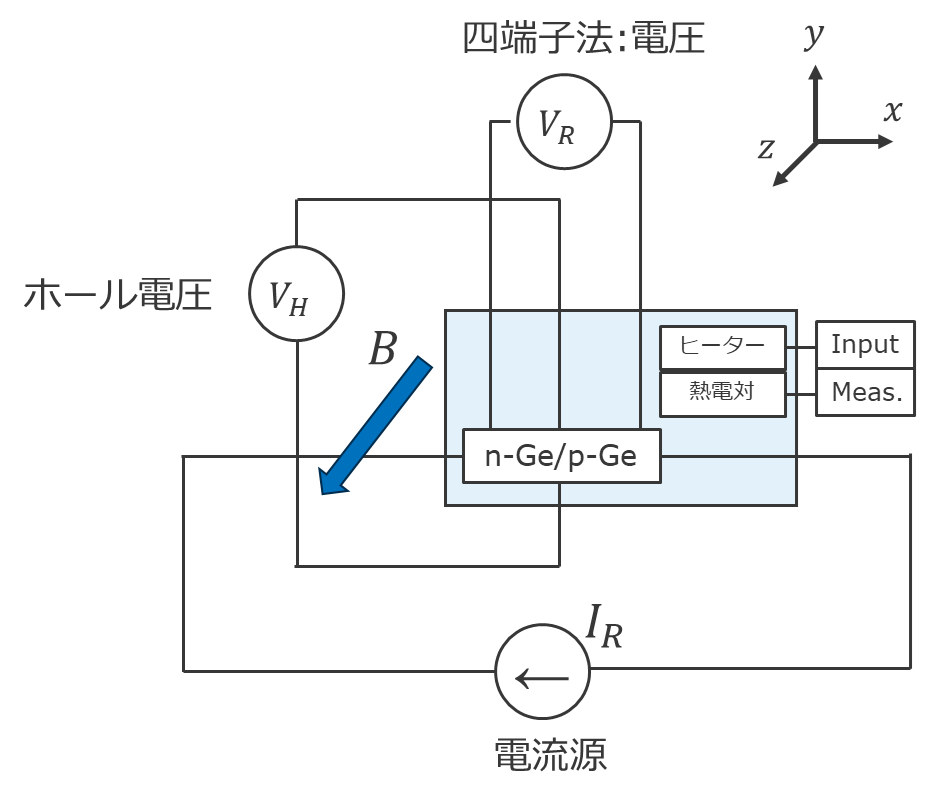
\includegraphics[width=0.4\columnwidth]{fig/fig02.png}
	\caption{測定装置の模式図。ホール電圧を測定するため\(y\)軸方向に端子をつけホール電圧を測定し、
	四端子法で電気伝導度を測定する。過熱をするためのヒーターと温度計として熱電対も装置に組み込まれている。}
	\label{fig:02}
\end{wrapfigure}
\ce{n-Ge}と\ce{p-Ge}の電気伝導にかかわるパラメーターとして電気伝導度と磁場をかけたときのホール係数を試料の温度を変えながら測定した。
測定装置の模式図は図\ref{fig:02}の通りである。
半導体の電気伝導度を測定するには接触抵抗やショットキー障壁といった要素を取り除くため、4端子法で行う。
また、電流を流す方向を\(x\)軸としたときホール電圧を測定する方向を\(y\)軸として、\(z\)軸方向に電磁石によって磁場をかける。
このときホール電圧を測定する端子が\(x\)軸方向へのずれてしまうため、
測定したホール電圧はそのままではずれが生じていることに注意する必要がある。
手順としては、電流を流したときの電磁石の出す磁束密度と電流の関係の校正を行ったのち、
試料のホール電圧の\(x\)軸方向への端子位置のずれを測定するため
-2.4 mA から 2.4 mAの直流電流を流しとゼロ磁場、室温の下で
電気伝導度とホール係数を測定した。
その後、同じ電流の範囲で \(\pm\)50 mT, \(\pm\)100 mT の磁場をかけた下でのホール電圧を測定した。
室温での測定が終わったら、ヒーターを付け試料の温度を上げていく。
1 mA の電流を試料に流しながら、ホール電圧と電気伝導度を測定した。
このとき試料のホール電圧の\(x\)軸方向への端子位置のずれの影響も考慮するため、
ゼロ磁場と 100 mT の磁場をかけたときの両方のホール電圧を測定する必要がある。

\section{結果}

\clearpage
\section{考察}
\subsection{素励起と準粒子}
結晶中の電子の振舞いについて考える。
1つの孤立している原子を考える。
電子はその原子核に束縛され、離散的なエネルギー準位をとるようになる。
その原子が2つ近づくと、相互作用により元のエネルギー準位が分裂して2つのエネルギー準位をとるようになる。
固体中であるためこのような相互作用が多数あるため、分裂したエネルギー準位はほとんど連続的なものとみなすことができる。
これがバンドである。

そうしたバンドの準位に電子は低いエネルギーから入っていく。
その際、
パウリの排他原理によりエネルギーの低い状態となっている電子は外乱により別の状態に遷移しようとしても、
すでにほかの電子がその状態を占めているため、状態を変えることが禁じられる。
一方、エネルギーの最も高い状態付近(フェルミ面)の電子は外乱により別の状態に遷移する際に、
フェルミ面より高い準位や、他の電子がすでに励起して空になったエネルギー準位遷移することができる。

これより、結晶に外乱をいれたときに応答に関わってくるのはフェルミ面付近だけ考えばよくなる。
これはもっと言うと、フェルミ面内部にある電子は系の応答に関わらないため無視をして、
励起によりフェルミ面の外に出た電子や空になった準位だけを考えることができる。
つまり、結晶の現象はフェルミ面を新たな真空として、その真空で対生成・対消滅する電子と正の電荷をもった孔(正孔)によるものだということができる。
このような描像を素励起といい、これらにより生成・消滅する粒子を準粒子というように呼ばれる。

\begin{wrapfigure}{r}[0pt]{0.4\columnwidth}
	\centering
	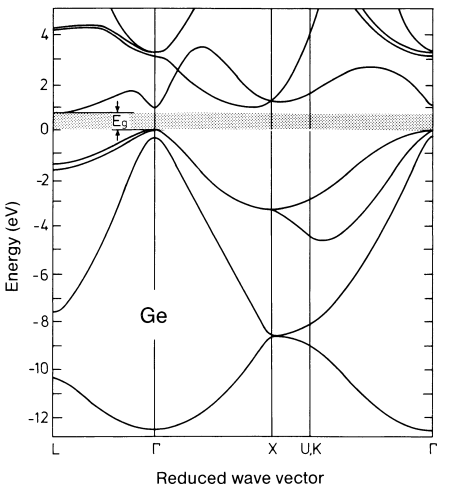
\includegraphics[width=0.4\columnwidth]{graph/graph01.png}
	\caption{Ge のバンド図\cite{ibach-luth}}
	\label{graph:01}
\end{wrapfigure}
この描像では結晶を構成する原子核の周期的ポテンシャルというのは、
準粒子の質量に取り込まれる。
このように周期的ポテンシャルを取り込んだ質量を有効質量と呼ぶ。
そのため準粒子としての電子は、
同じ電子という名前が付いているが実態としては真空中の電子とは異なり、
一定の質量をもたないような別の粒子になっている。
正孔というのも名前に孔というようにあるが、しっかりと(有効)質量をもった粒子とみなす。

有効質量は定量的にはバンドの曲率として定義される。
つまり
\begin{equation}
	\frac{1}{m_{ij}} = \pdv[2]{E(\vb*{k})}{k_i}{k_j}
\end{equation}
として定義される。
波数空間が等方的であるときには有効質量はテンソル量ではないスカラー量
\begin{equation}
	\frac{1}{m} = \pdv[2]{E(\vb*{k})}{k}
\end{equation}
となる。
有効質量によって周期的ポテンシャルというのは準粒子の運動方程式に現れなくなり、
自由粒子と同じ運動方程式となる。なので準粒子は固体内部で理想気体のように振舞う。

実際の Ge のバンド図(図\ref{graph:01})との対応を見てみる。
フェルミ面がバンドギャップ\(E_g\)の間を通っている結晶は半導体と呼ばれる。
実際に電子と正孔の対生成・対消滅する場所としては Reduced wave vector が \(\Gamma\)
つまり波数ベクトルが\(\vb*{k}=(0,\,0,\,0)\)の地点にあるエネルギーギャップ付近である。
上下に放物線があり、上にある放物線上に準粒子としての電子が現れ、下にある放物線上に正孔が現れる。
このとき正孔は真空より低い負のエネルギーを持っているように見えるが、
そのようにとらえるのではなく符号を取り直して正のエネルギーを持つものと考える。
\footnote{Dirac が考えた Dirac の海による陽電子の説明と似ている。
歴史的には Peierls が1929年に電子と正孔を用いて Holl 効果を説明してから Dirac の海の話が1930年に出たようである。
Dirac の海による陽電子の予言の偉いところは Dirac の海のような描像を思いつた点ではなく、
電子と正孔の生成というのがフェルミ面という"真空"で粒子が対生成・対消滅していて、
真空でもこれと同様なことを思いついた点であるのだろう。ただこの話の証拠はないため私の妄想ではある。}
フェルミ面を真空としているので、フェルミ面のエネルギーを 0 とすると\footnote{図\ref{graph:01}の縦軸のエネルギーの基準点とは違う基準}、
この放物線はそれぞれ、
\begin{equation}
	E(k) = E_e + \frac{\hbar^2k2}{2m_e^*}, \qquad
	E(k) = -\qty(E_p + \frac{\hbar^2k2}{2m_p^*})
\end{equation}
となる。ここで\(E_e,\,E_p\)を電子と正孔の生成エネルギー、\(m_e^*,\,m_p^*\)を電子と正孔の有効質量とした。
電子・正孔の分散関係と呼ばれ、分散関係がわかるとエネルギーの幅が\([E,\,E+dE]\)の間にとることのできる状態の数を表す(有効)状態密度\(D(E)dE\)というのも求められる。

エネルギー\(E(k)\)における状態密度は粒子の生成エネルギーを\(E_s\)として
\begin{align}
	D(E)
	&= 2\times\sum_k \delta(E-E(k)) \notag\\
	&= \frac{2V}{(2\pi^3)}\int d\vb*{k}\, \delta\qty(E-E_s - \frac{\hbar^2k^2}{2m^*}) \notag\\
	&= \frac{V}{\pi^2} \int dk\, k^2\times \frac{1}{2}\sqrt{\frac{\hbar^2}{2m^*(E-E_e)}}\qty{\delta\qty(k-\sqrt{\frac{2m^*(E-E_s)}{\hbar^2}})+\delta\qty(k+\sqrt{\frac{2m^*(E-E_s)}{\hbar^2}})} \notag\\
	&= \frac{V}{2\pi^2}\qty(\frac{2m^*}{\hbar^2})^{3/2}\sqrt{E-E_s}
\end{align}
として求められる。

また、粒子の分布関数はフェルミ分布関数で表される。
しかし、\(E_e,\, E_p \simeq \text{eV} \simeq 10^4 \text{K}\)であることから、
\num{e4} K のような高温でない限り、フェルミ分布関数をボルツマン分布とみなしてよい。
\begin{equation}
	f(E) = \frac{1}{1+e^{E/k_BT}} \simeq e^{-E/k_BT}
\end{equation}
これより電子と正孔の密度は
\begin{align}
	n &= \int_{E_e}^\infty D_e(E) f(E) dE = 2\qty(\frac{m_e^*k_BT}{2\pi\hbar})^{3/2}e^{-E_e/k_BT}\\
	p &= \int_{E_p}^\infty D_p(E) f(E) dE = 2\qty(\frac{m_p^*k_BT}{2\pi\hbar})^{3/2}e^{-E_p/k_BT}
\end{align}
となる。
この式から質量作用の法則と呼ばれる式
\begin{equation}
	pn = 4\qty(\frac{k_B T}{2\pi\hbar})^3\qty(m_p^*m_n^*)^{3/2} e^{-E_g/k_BT}
\end{equation}
が得られる。
結晶内での電荷中性条件\(p=n\)より
\begin{equation}
	p=n=2\qty(\frac{k_B T}{2\pi\hbar})^{3/2}\qty(m_p^*m_n^*)^{3/4} e^{-E_g/2k_BT}
\end{equation}
が得られる。
電荷中性条件から別の式を得ることができる。
\(p/n=1\)より
\begin{align}
	1 &= \qty(\frac{m_p^*}{m_e^*})^{3/2}e^{-(E_p-E_c)/k_BT}\\
	E_p - E_n &= \frac{3}{2}k_BT\ln(\frac{m_p^*}{m_e^*})
\end{align}
\(E_g = E_p + E_n\)と合わせて考えると
\begin{equation}
	E_p = \frac{E_g}{2} + \frac{3}{4}k_BT\ln(\frac{m_p^*}{m_e^*}), \qquad
	E_n = \frac{E_g}{2} + \frac{3}{4}k_BT\ln(\frac{m_n^*}{m_p^*})
\end{equation}
という式が得られる。
低温であれば\(E_p=E_n=E_g/2\)であることがわかり、
温度を上げていくと有効質量の大小によって正孔と電子の生成エネルギーに差ができることがわかる。
\ce{Ge}ではバンド図(図\ref{graph:01})より\(m_e^* < m_p^*\)であるため正孔の方が大きい。

通常のバンド理論ではフェルミ面より下にあるバンドを価電子帯、上にある伝導帯と呼ばれる。
この呼び方は次のような描像から来ている。
価電子帯と呼ばれるバンドの内部にある電子は、
上の説明からわかるように電気伝導にかかわることはない。
その理由をこの電子は原子核に束縛されて動けない価電子であるからだというように考える。
一方、伝導体と呼ばれるバンドの内部にある電子は素励起による説明における電子になっている。
するとその電子は束縛されていない自由電子で、結晶内を移動していくキャリアとなる。
なので価電子帯や伝導帯のように呼ばれている。
また、正孔にとってはフェルミ面の上側にあるのが価電子帯、下側にあるのが伝導帯となる。

\subsection{半導体への不純物ドーピング}
Ge 半導体に原子番号が隣の元素である \ce{As} か \ce{Ga} の一方を少量だけ混ぜることを考える。
まず初めに \ce{As} を1つだけ加えることを考える。
素励起の描像では \ce{Ge} の結晶だけでは真空であったので、
もともとの \ce{Ge} 結晶からの差分だけが系にあるとみなせる。
\ce{As} の原子核の持つ正電荷は\ce{Ge}の原子核と比較するとだいたい1つ増え、電子が1つ増える。
つまり水素原子と同じ系になっている。
よって新しく追加された電子のシュレーディンガー方程式は
\begin{equation}
	\qty(-\frac{\hbar^2}{2m_e^*}\laplacian - \frac{e^2}{4\pi\varepsilon r})\psi = E \psi
\end{equation}
となる。ここで、\(\varepsilon\)は\ce{Ge}結晶の誘電率である。
\ce{As} に束縛された電子は\ce{Ge}の電子の分散曲線に励起すると自由電子となることから、
エネルギーは伝導体の下端をエネルギーの基準とした
\begin{equation}
	E_n = E_e - \frac{m_e^*}{2\hbar^2}\qty(\frac{e^2}{4\pi \varepsilon})^2\frac{1}{n^2}
\end{equation}
というようになる。
追加する不純物は少量であるため、不純物間の間は十分離れてるとみなせる。
なのでこれによるバンド分裂は細くてないものとみなせる。
もともとのエネルギーは eV オーダーの量にたいして、
不純物によってできた新たな準位による束縛エネルギーは meV オーダーである。
これより極端な低温ではないかぎり、熱よって励起をすることができる。
そうして熱励起した電子はキャリアとして半導体内を動くようになる。
なのでキャリアの符号からこれをn型半導体という。

そして\ce{Ga}を加えたときのことを考える。
もともとの \ce{Ge} 結晶からの差分だけが系にあるとみなせる。
\ce{Ga} の原子核の持つ正電荷は\ce{Ge}の原子核と比較するとだいたい1つ減り、電子が1つ減る。
これはつまり、負の電荷をもった原子核の周りに正の電荷をもった正孔があるという水素原子と同じ系となる。
なので\ce{As}のときと同様に考えて
\begin{equation}
	E_n = E_p - \frac{m_e^*}{2\hbar^2}\qty(\frac{e^2}{4\pi \varepsilon})^2\frac{1}{n^2}
\end{equation}
というようなエネルギー準位が表れ、
熱により、正孔がキャリアとして励起することができる。
これをp型半導体という。

不純物が入っていない半導体を真性半導体という。
これら3つの簡略化したバンド図は図\ref{fig:01}のようになる。 % TODO もっと説明書く
\begin{figure}[h]
	\centering
	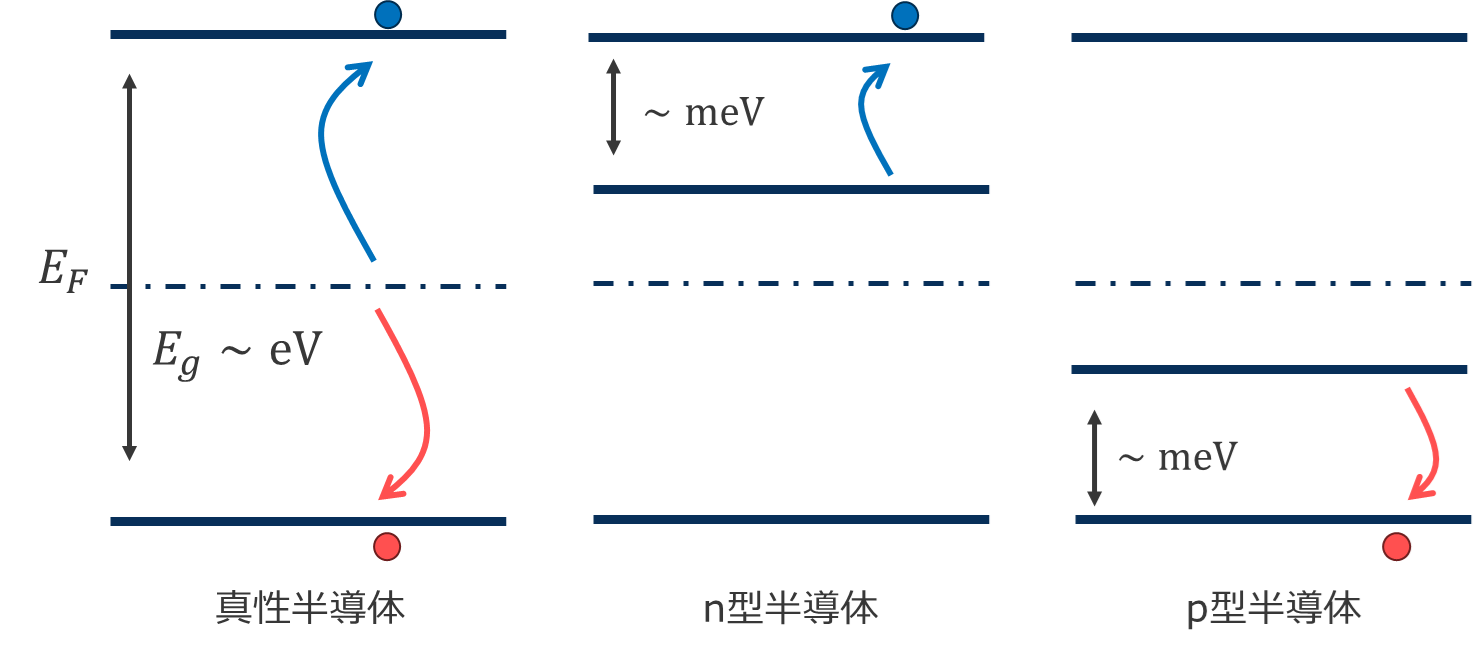
\includegraphics[width=0.65\columnwidth]{fig/fig01.png}
	\caption{不純物を入れたときの簡略化したフェルミ面付近のバンド図}
	\label{fig:01}
\end{figure}

\section{結論}


\bibliographystyle{junsrt}
\bibliography{reference}
\section*{付録}

\end{document}